% Defining string as labels of certain blocks.
\newcommand{\suma}{\Large$+$}
\newcommand{\inte}{$\displaystyle \int$}
\newcommand{\derv}{\huge$\frac{d}{dt}$}

\resizebox{.5\textwidth}{!}{
    \begin{tikzpicture}
        \begin{small} 
            \sbEntree{E}
            \sbBloc[4]{algo}{Algo.}{E}
            \sbRelier[$w(k)$]{E}{algo}
            \sbBloc[4]{conv1}{D/A}{algo}
            \sbRelier[$u(k)$]{algo}{conv1}
            \sbBloc[4]{sys}{Sys.regl.}{conv1}
            \sbRelier[$u(t)$]{conv1}{sys}
            \sbSortie[4]{S}{sys}
            \sbRelier[$y(t)$]{sys}{S}
            \sbDecaleNoeudy[4]{S}{U}
            \sbBlocr[12.1]{conv2}{A/D}{U}
            \sbRelieryx{sys-S}{conv2}
            \sbRelierxy[$y(k)$]{conv2}{algo}      
        \node[draw] at (4.8,-2.5) { Retard total : $T_r  =  T_{cal} + T_{convAD} + T_{convAD} + T_{rec} \approx h $};   
        \draw [-latex,red,thick] (3.5,-2.3) to [out=90,in=330] (algo);
        \draw [-latex,blue,thick] (5.3,-2.3) to [out=90,in=320] (conv2);
        \draw [-latex,green!50!black,thick] (6.5,-2.3) to [out=90,in=310] (conv1);
        \draw [-latex,teal!80!purple,thick] (8,-2.3) to [out=90,in=330] (conv1);   
    \end{small}
    \end{tikzpicture}
}

\vspace{3mm}

Ce qui est approximable avec un retard pur par : 

\vspace{3mm}

\begin{tikzpicture}
    \begin{small} 
            \sbEntree{E}
            \sbBloc[4]{algo}{$G_c(S)$}{E}
            \sbRelier[$w(k)$]{E}{algo}
            \sbBloc[4]{conv1}{$e^{-sh}$}{algo}
            \sbRelier[$u(k)$]{algo}{conv1}
            \sbBloc[4]{sys}{$G_a(S)$}{conv1}
            \sbRelier[$u(t)$]{conv1}{sys}
            \sbSortie[4]{S}{sys}
            \sbRelier[$y(t)$]{sys}{S}
            \sbRenvoi{sys-S}{algo}{}
    \end{small}
\end{tikzpicture}